%*****************************************
\chapter[BaldWhisper]{BaldWhisper: Faster Whisper with Head Shearing and Layer Merging}\label{ch:baldwhisper}
%*****************************************

\section{Introduction}

In the previsous chapter we showed that our proposed low-rank compression significantly speedup the \textit{Time to First Token} (TTF), i.e., the \textit{prefiling phase} while still maintaining most of the base performance.
However the method shows limited speedup the end-to-end \textit{decoding} latency. For example, on Whisper the overall latency speedup is only $1.13\times$.
This is because autoregressive decoding is mostly \textit{memory-bound}. At each decoding step, the model processes only a single token. Instead, the dominant cost comes from repeatedly loading the model weights and KV-cache from GPU memory. 
Since memory bandwidth, rather than compute throughput, becomes the limiting factor, reducing the number of arithmetic operations in the linear layers alone has only a modest impact on decoding latency.
We can also notice that the low-rank architecture can further introduce memory bandwith bottleneck since instead of a single linear matrix multiplication $xW$ we do $(xW_{1})W_{2}$. 
This further introduces intermediate activations and data movement. Specific GPU kernels
are needed to achieve substantial speedup with this compression approach.

To further accelerate end-to-end inference without any GPU kernel, we need to reduce not only the computational complexity of the model but also the amount of data transferred from memory.
Motivated by these observations, this chapter introduces a compression method that achieve substantial speedup by combining low-rank compression and layer merging to reduce the number of KV-cache layers, 
leading to significantly larger end-to-end speedups. The method, named \emph{BaldWhisper}, is a two-stage decoder compression method designed to preserve accuracy in the data-scarce setting.
First, we reduce the decoder depth which lowers weight traffic and reduces the number of key--value cache layers used during generation. Second, we compress Whisper's shared input/output embedding matrix through activation-aware low-rank decomposition.
This matrix accounts for more than half of the decoder parameters in small multilingual Whisper models.

Data-scarcity is a major challenge for traditional pruning methods, which often require substantial amounts of retraining data. For example, Distill-Whisper \citep{distill-whisper} prunes the English-only version of Whisper \citep{whisper} and further retrained on 21k hours of ASR data, a quantity not available for many languages. This leads us to a central question: \emph{How to compress a pre-trained ASR model (Whisper) when only a small quantity of supervised data is available?}
We study this questin through the compression of Whisper for Bambara, a low-resource language with limited amount of ASR dataset at the time of this work. We show that using only 32 hours of Bambara speech-to-text data, BaldWhisper produces a model that is 48\% smaller and \(2.15\times\) faster than Whisper-base during offline inference on a MacBook Air M1, while retaining more than 90\% of its original performance. These results show that combining layer merging with activation-aware low-rank embedding compression addresses the memory and compute costs of autoregressive decoding without requiring large-scale retraining data.

\begin{figure}[ht]
    \centering
    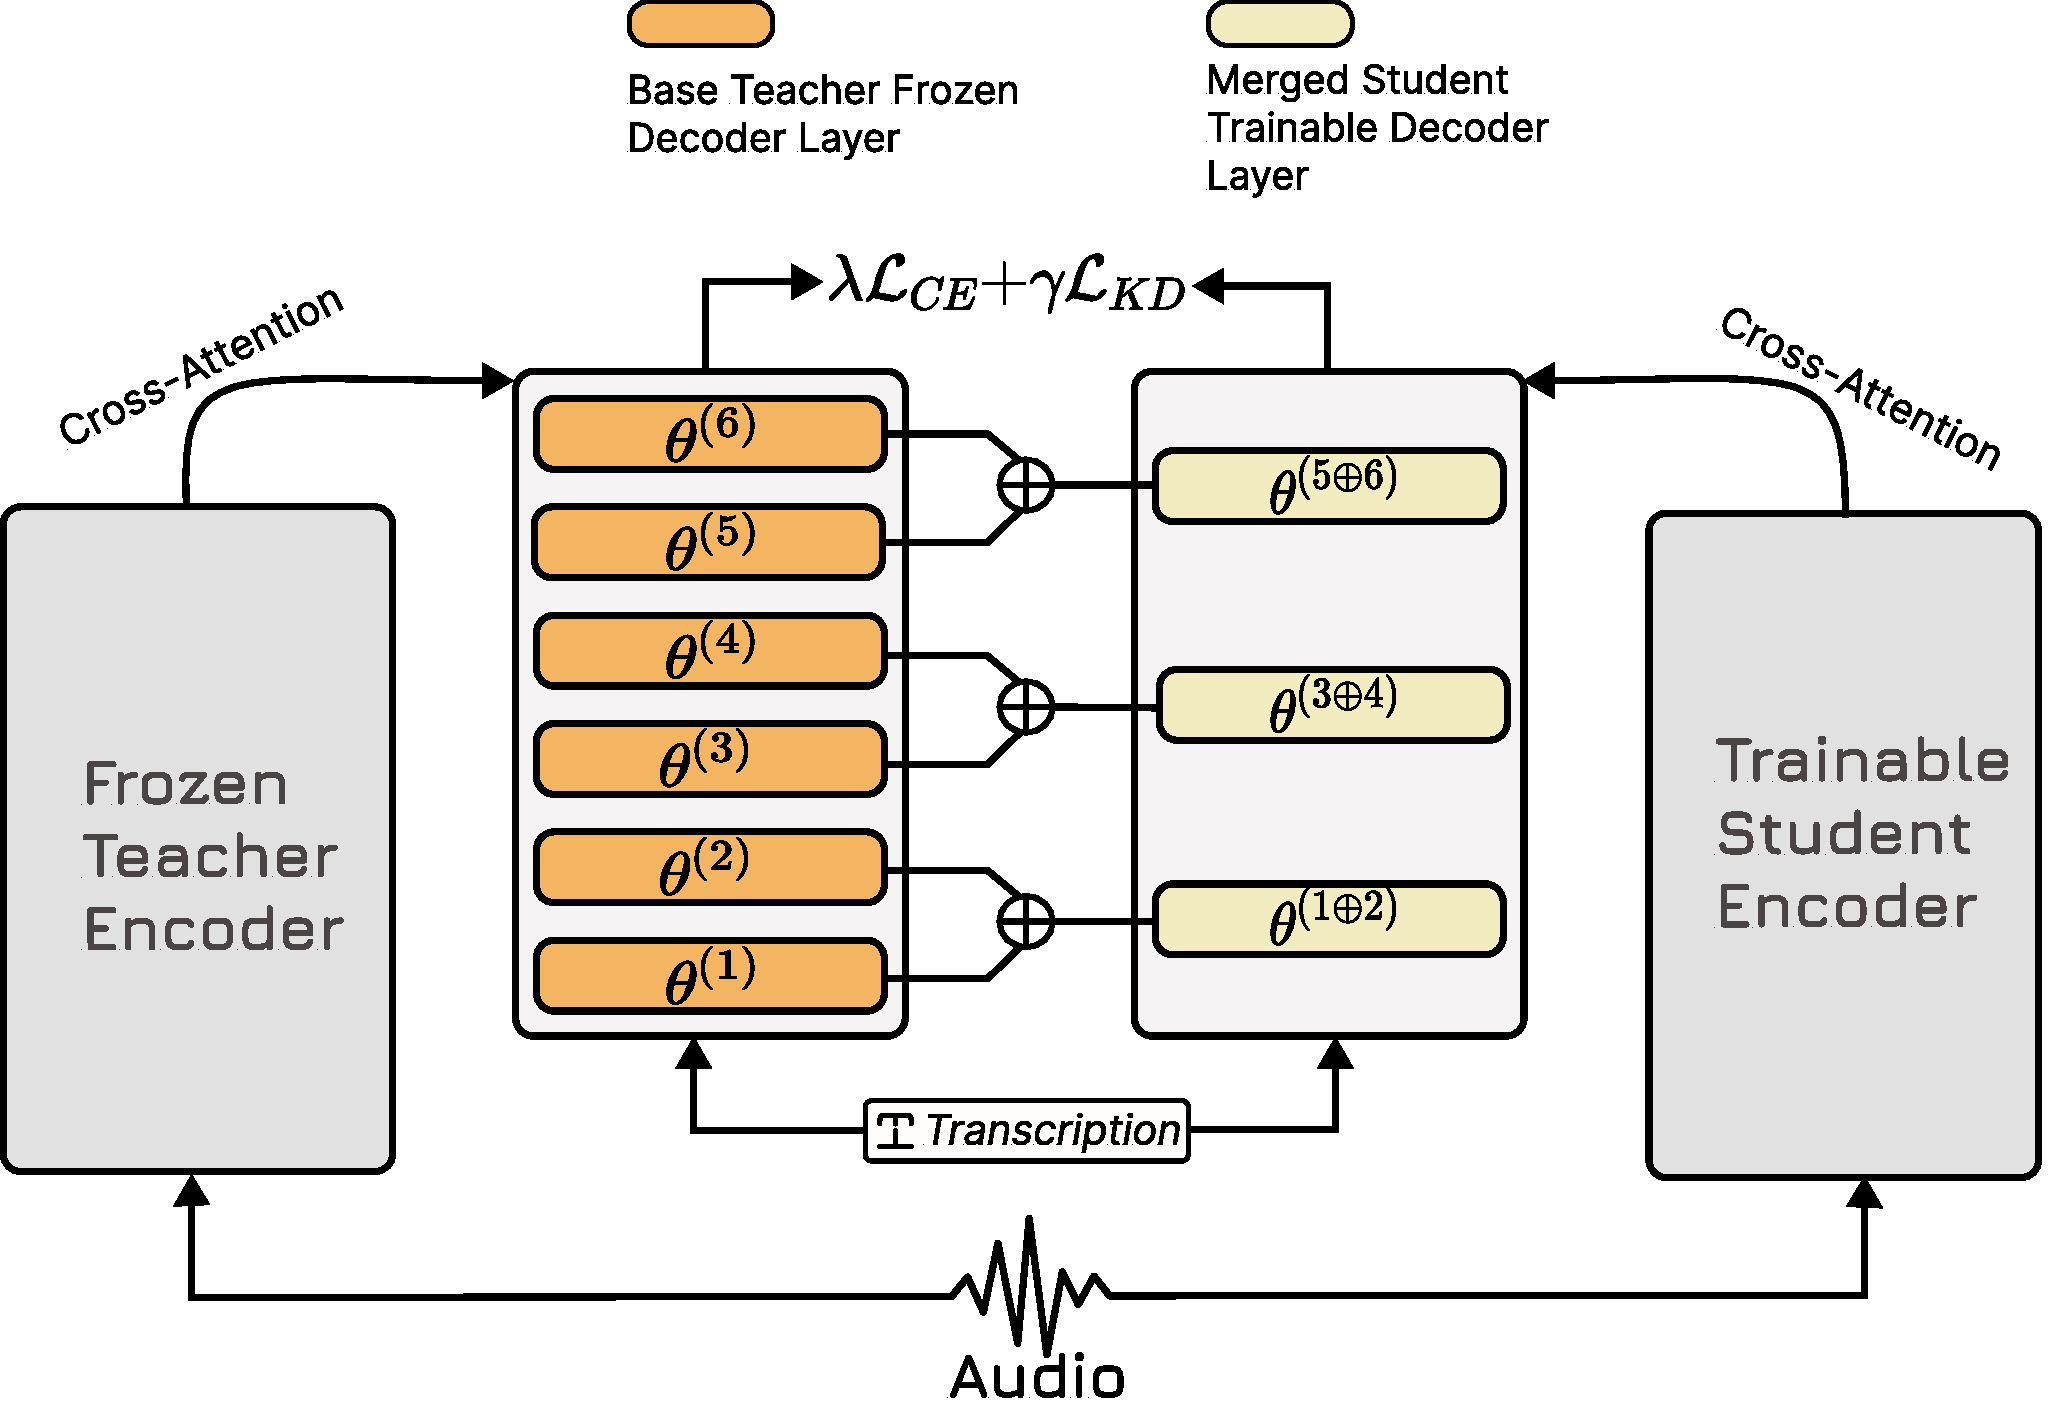
\includegraphics[width=1.0\textwidth]{papers/BaldWhisper/images/layermerging.pdf}
    \caption{Layer merging in the Whisper decoder: each student layer is a weighted average of two consecutive teacher layers, then trained with cross-entropy and knowledge distillation.}
    \label{fig:layermerging-bw}
\end{figure}

Before presenting our method, we discuss some approaches related to this work.

\paragraph{Deep encoder, shallow decoder.}
We take inspiration from \citep{kasai2021deepencodershallowdecoder}, who show that the decoder part of an encoder--decoder architecture can be very shallow while remaining accurate and becoming faster. We likewise compress primarily the decoder of Whisper. In contrast to their approach, which trains encoder--decoder models from scratch, we begin with a pretrained Whisper model and compress its decoder.

\paragraph{Distil-Whisper.}
Distil-Whisper~\citep{distill-whisper} compresses Whisper-large by removing 30 of its 32 decoder layers. The pruned model is then retrained on approximately 21,000 hours of speech using sequence-level knowledge distillation~\citep{kim2016sequence}. Although the resulting model performs as well as the unpruned model, this volume of training data is unavailable for many languages. Instead of removing layers, we merge them to limit the performance loss.

\paragraph{Model merging.}
Our decoder compression is related to model-merging approaches used either to combine models trained for different tasks~\citep{wortsman2022modelsoupsaveragingweights,yadav2023tiesmergingresolvinginterferencemerging} or to reduce model size~\citep{liu2024pruningmergingcompressingllms}. The latter method uses manifold learning to align activations before merging layers. BaldWhisper uses a simpler procedure: motivated by the similarity of adjacent-layer activations, it compresses the decoder through a weighted average of adjacent layers. We study different weighting values and find that assigning greater weight to the upper layer produces better results.

\paragraph{Vocabulary pruning.}
In small multilingual models, the embedding matrix accounts for a large proportion of the parameters because of the multilingual vocabulary. In Whisper-tiny, for instance, this matrix represents 51\% of all parameters. Vocabulary pruning~\citep{abdaoui-etal-2020-load,vocabprune} removes tokens not used in the target language, but it is risky in the presence of out-of-vocabulary words and code-switching, where foreign-language tokens must remain available. Bambara speakers, for example, frequently mix French in francophone regions such as Mali and English in anglophone regions such as The Gambia. We therefore replace vocabulary pruning with low-rank decomposition and feature distillation.

\paragraph{Low-rank decomposition.}
Low-rank decomposition is a common dimensionality-reduction technique. Recent work has shown that pretrained Transformer activations are low-rank, motivating activation-aware low-rank decomposition~\citep{yu_compressing_2023,chen_drone}. Whisper's embedding matrix is particularly large because of its multilingual vocabulary. We compress it using activation information rather than relying only on a standard SVD, training the low-rank embeddings through gradient-based feature distillation.

\section{BaldWhisper Approach}
\label{sec:method-bw}

\begin{figure}[ht]
    \centering
    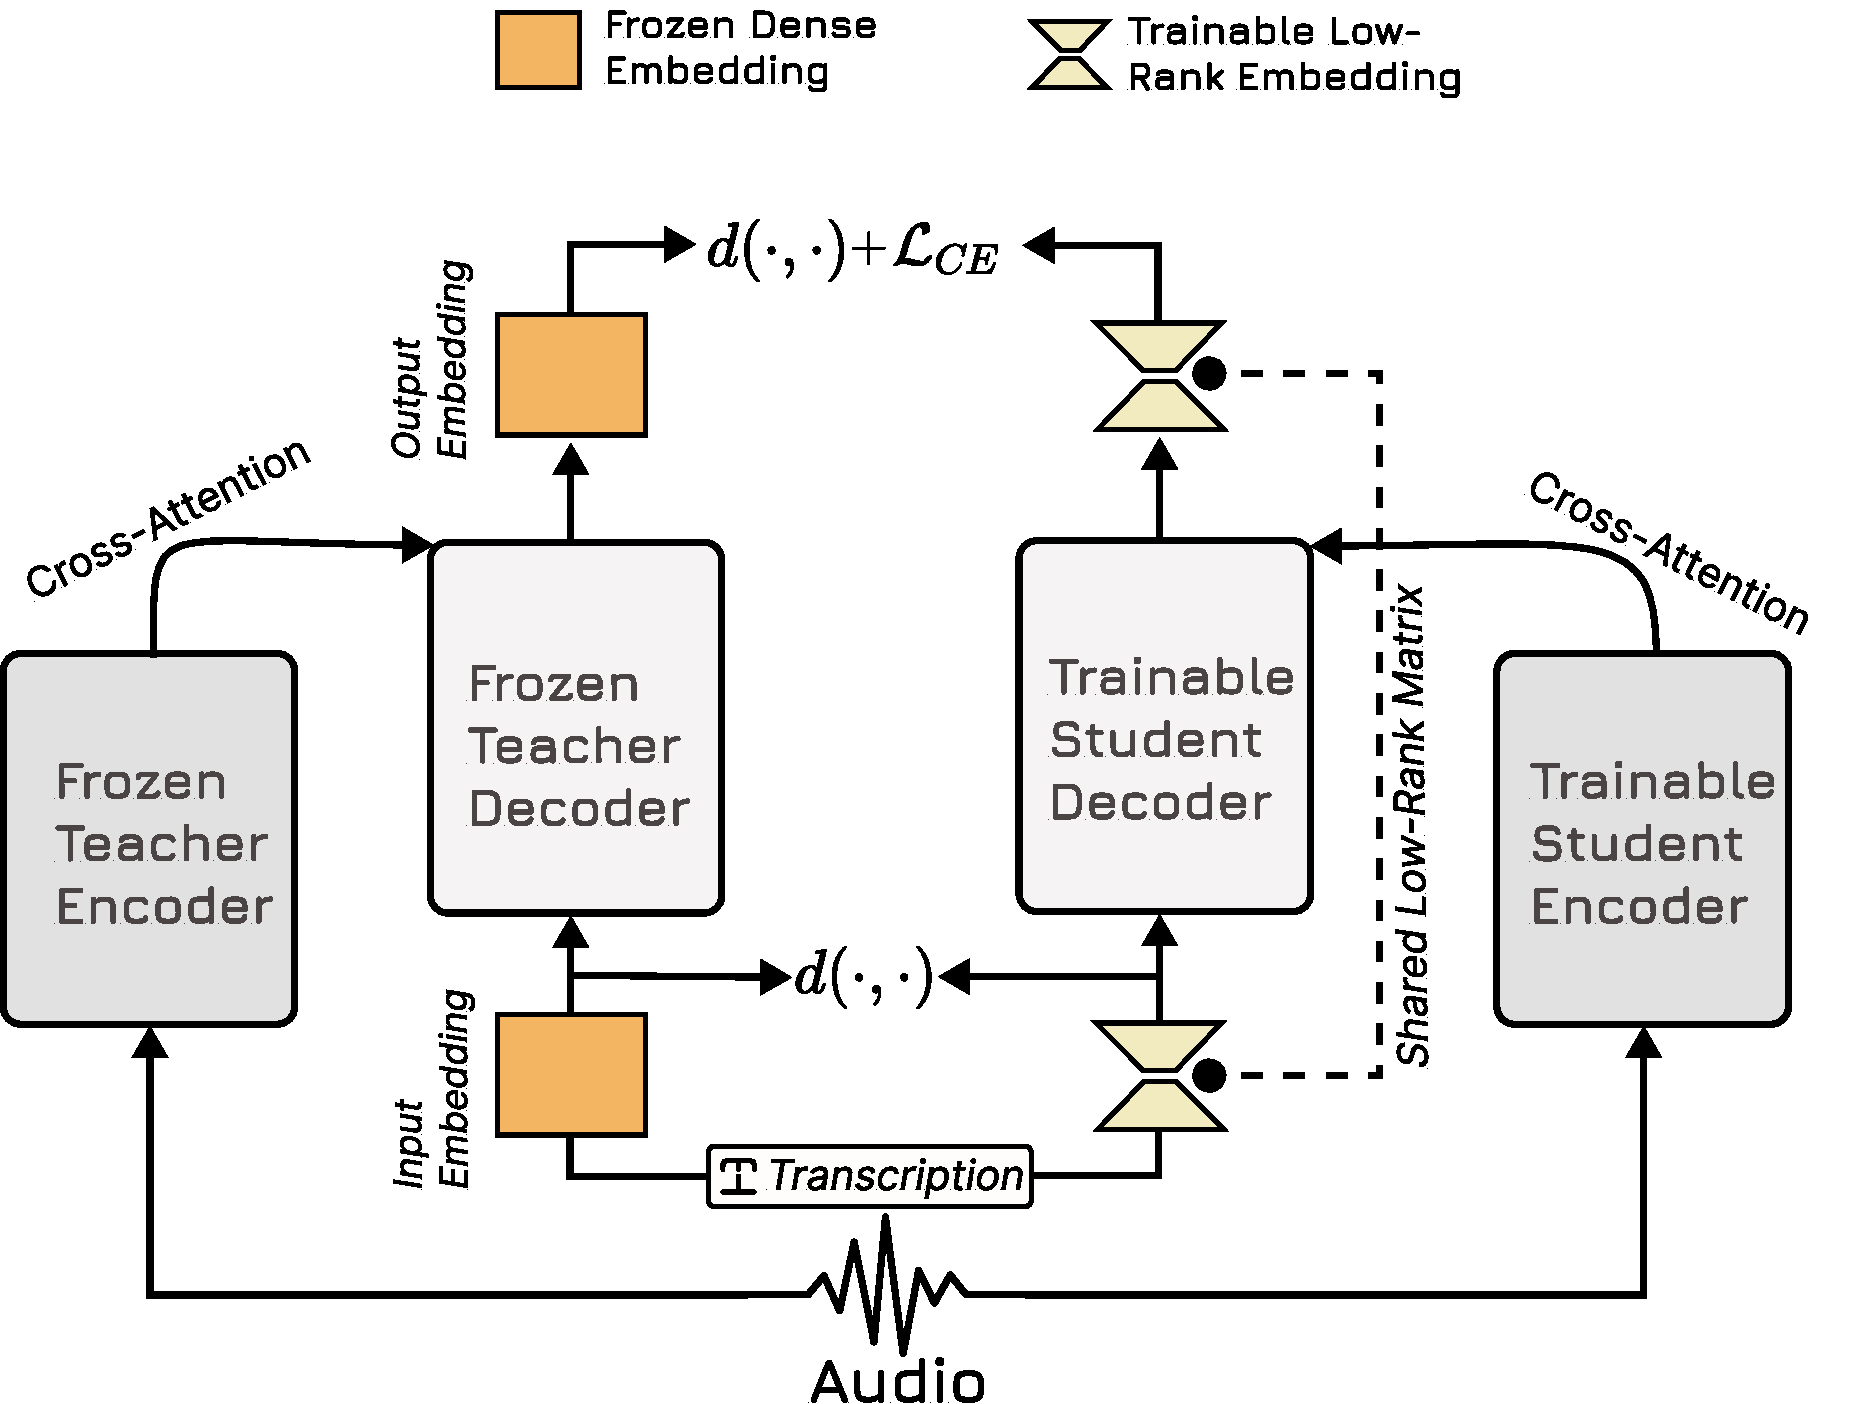
\includegraphics[width=1.0\textwidth]{papers/BaldWhisper/images/headshearing.pdf}
    \caption{Head shearing of the Whisper embedding through low-rank decomposition. The decomposition is activation-aware because the low-rank weights are subsequently feature-distilled.}
    \label{fig:headshearing-bw}
\end{figure}

\paragraph{Motivation.}
We target offline, on-device decoding. Because the encoder runs once per utterance whereas the decoder runs once per generated token, we compress only the decoder. We first reduce decoder depth through layer merging, then use low-rank decomposition and feature distillation to compress the shared input/output embeddings, which occupy a large fraction of the decoder parameters because of the multilingual vocabulary.

\subsection{Stage 1: Layer Merging}

To accelerate inference with a minimal accuracy loss, we reduce the decoder depth by merging layers instead of removing them. Let \(\theta^{(l)}\) denote the parameters of layer \(l\). Figure~\ref{fig:layermerging-bw} illustrates this stage. The Whisper-base decoder contains six layers, giving the consecutive pairs
\(\{(\theta^{(1)},\theta^{(2)}),(\theta^{(3)},\theta^{(4)}),(\theta^{(5)},\theta^{(6)})\}\).
We merge each pair through a weighted average:
\begin{equation}
\label{eq:merge-bw}
\theta^{(i \oplus j)}
= \frac{\alpha \theta^{(i)} + \beta \theta^{(j)}}{\alpha + \beta},
\end{equation}
where \(j=i+1\), and \(\alpha\) and \(\beta\) control each layer's contribution. Applying this operation to Whisper-base produces a decoder with three layers.

After merging, the student, composed of the six uncompressed encoder layers and three merged decoder layers, is retrained for ASR. We also distill the compressed student from the frozen, uncompressed teacher, since distillation is effective for speech recognition~\citep{distillation,distill-whisper}. Only the student encoder and decoder are updated. The training objective is
\begin{equation}
    \label{eq:hs-bw}
    \mathcal{L}^{(1)} = \lambda \mathcal{L}_{\mathrm{CE}} + \gamma \mathcal{L}_{\mathrm{KD}},
\end{equation}
where \(\mathcal{L}_{\mathrm{CE}}\) is the student's cross-entropy loss for ASR and \(\mathcal{L}_{\mathrm{KD}}\) is the Kullback--Leibler divergence between the student and teacher predictions. The weights \(\lambda\) and \(\gamma\) are selected through hyperparameter search.

\subsection{Stage 2: Activation-Aware Embedding Decomposition}

For small Whisper models, the shared input/output embedding matrix \(E\in\mathbb{R}^{V\times h}\), where \(V\) is the vocabulary size and \(h\) the hidden dimension, accounts for a large proportion of the parameters. Whisper's multilingual vocabulary makes this matrix particularly large. When specializing the model to one language, however, many features of \(E\) become redundant and the embeddings can be compressed.

As illustrated in Figure~\ref{fig:headshearing-bw}, we first use SVD to factorize \(E\approx E_1E_2\), where \(E_1\in\mathbb{R}^{V\times r}\), \(E_2\in\mathbb{R}^{r\times h}\), and \(r\ll\min(V,h)\). To preserve the base embedding's features, we combine the ASR cross-entropy loss with feature-distillation objectives at both the input and output:
\begin{align}
    \label{eq:distill-bw}
    \mathcal{L}^{(2)}
    &= \mathcal{L}_{\mathrm{CE}} \nonumber \\
    &\quad + d(E[x], E_1[x]E_2) \nonumber \\
    &\quad + d(oE^{T}, (oE_2^{T})E_1^{T}),
\end{align}
where \(x\) is the input sequence, \(o\) is the output of the final decoder layer, and \(d(\cdot,\cdot)\) is the feature-distillation loss:
\begin{align}
    \label{eq:distance-bw}
    d(y,\hat{y})
    &= \mathcal{L}_{\ell_1}(y,\hat{y})+\mathcal{L}_{\cos}(y,\hat{y}) \nonumber\\
    &= \frac{1}{h}\sum_{i=1}^{h}|y_i-\hat{y}_i|
       -\log \sigma\!\left(\cos(y,\hat{y})\right).
\end{align}
Here, \(\sigma\) is the sigmoid function and \(\cos(\cdot,\cdot)\) is cosine similarity. Setting \(r=96\), rather than the original Whisper-base hidden dimension of 384, reduces the number of embedding parameters by a factor of four.

\section{Experiments}

\subsection{Experimental Setup}

\paragraph{Data.}
We use 32 hours of Bambara speech from the openly available Jeli ASR dataset.\footnote{\url{https://huggingface.co/datasets/RobotsMali/jeli-asr}} We reserve 50 minutes for development and 1 hour 20 minutes for testing, using the remainder for training.

\paragraph{Implementation details.}
We first fine-tune the 73M-parameter Whisper-base model on the Bambara dataset for 20 epochs on one A100 80GB GPU with a learning rate of \(5\times10^{-5}\). We then compress it using the two stages described in Section~\ref{sec:method-bw}. For Stage~1, Bayesian optimization selects the merging weights \(\alpha\) and \(\beta\) that minimize development-set WER. We run 30 search iterations using Ax.\footnote{\url{https://ax.dev/}} The merged model is then fine-tuned with the objective in Equation~\ref{eq:hs-bw}. We independently tune \(\lambda\) and \(\gamma\) and use a learnable temperature in the Kullback--Leibler divergence. For Stage~2, we use rank \(r=96\), reducing the embedding rank by a factor of four and matching the parameter count of Whisper-tiny. The model with low-rank input/output embeddings is then fine-tuned with Equation~\ref{eq:distill-bw}.

\subsection{Results}

\begin{table}[ht]
    \centering
    \begin{tabular}{lccc}
    \toprule
    \textbf{Model} & \textbf{Params (M)} & \textbf{Speed (tokens/s)} & \textbf{WER (\(\downarrow\))} \\
    \midrule
    Whisper-base & 73 & 66.57 & 33.11 \\
    \(+\) Layer Merging & 60 & 102.24 & 34.77 \\
    \(+\) Head Shearing & 38 & 142.82 & 36.49 \\
    \bottomrule
    \end{tabular}
    \caption{\textbf{Main results.} Accuracy and efficiency after layer merging and head shearing (embedding decomposition). Speed is measured on a MacBook Air M1 while decoding 256 tokens for each utterance in a batch of 10. Bambara's less standardized orthography may partly explain the high absolute WER.}
    \label{tab:results-bw}
\end{table}

\paragraph{Performance.}
Table~\ref{tab:results-bw} summarizes both compression stages. Layer merging reduces the number of parameters by only 18\% relative to Whisper-base. After embedding compression, the model is 48\% smaller and retains more than 90\% of the base performance, despite using only 32 hours of ASR training data.

\paragraph{Speedup.}
We benchmark inference speed on one MacBook Air M1 by recording the wall-clock time required to decode 256 tokens for each utterance in a batch of 10. The layer-merged model is \(1.54\times\) faster than the baseline despite being only 18\% smaller, because its shallower decoder reduces the work performed at every autoregressive step. Adding embedding compression increases the speedup to \(2.15\times\).

\paragraph{Comparison with Whisper-tiny.}
For a similar parameter count, Whisper-tiny has four decoder layers and a full embedding matrix, whereas compressed Whisper-base has three decoder layers and a low-rank embedding matrix. Our compressed model generates 142.82 tokens per second, compared with 116.24 tokens per second for Whisper-tiny.

\section{Analysis}

\paragraph{How should \(\alpha\) and \(\beta\) be chosen?}
We use Bayesian optimization to select the merging weights \(\alpha\), which controls the lower layer's contribution, and \(\beta\), which controls the upper layer's contribution. Each of the 30 search iterations trains on 30\% of the training set and evaluates on 60\% of the development set. Figure~\ref{fig:convergence-bw} provides empirical support for the resulting settings: the lower layer should consistently receive less weight.

\begin{figure}[ht]
    \centering
    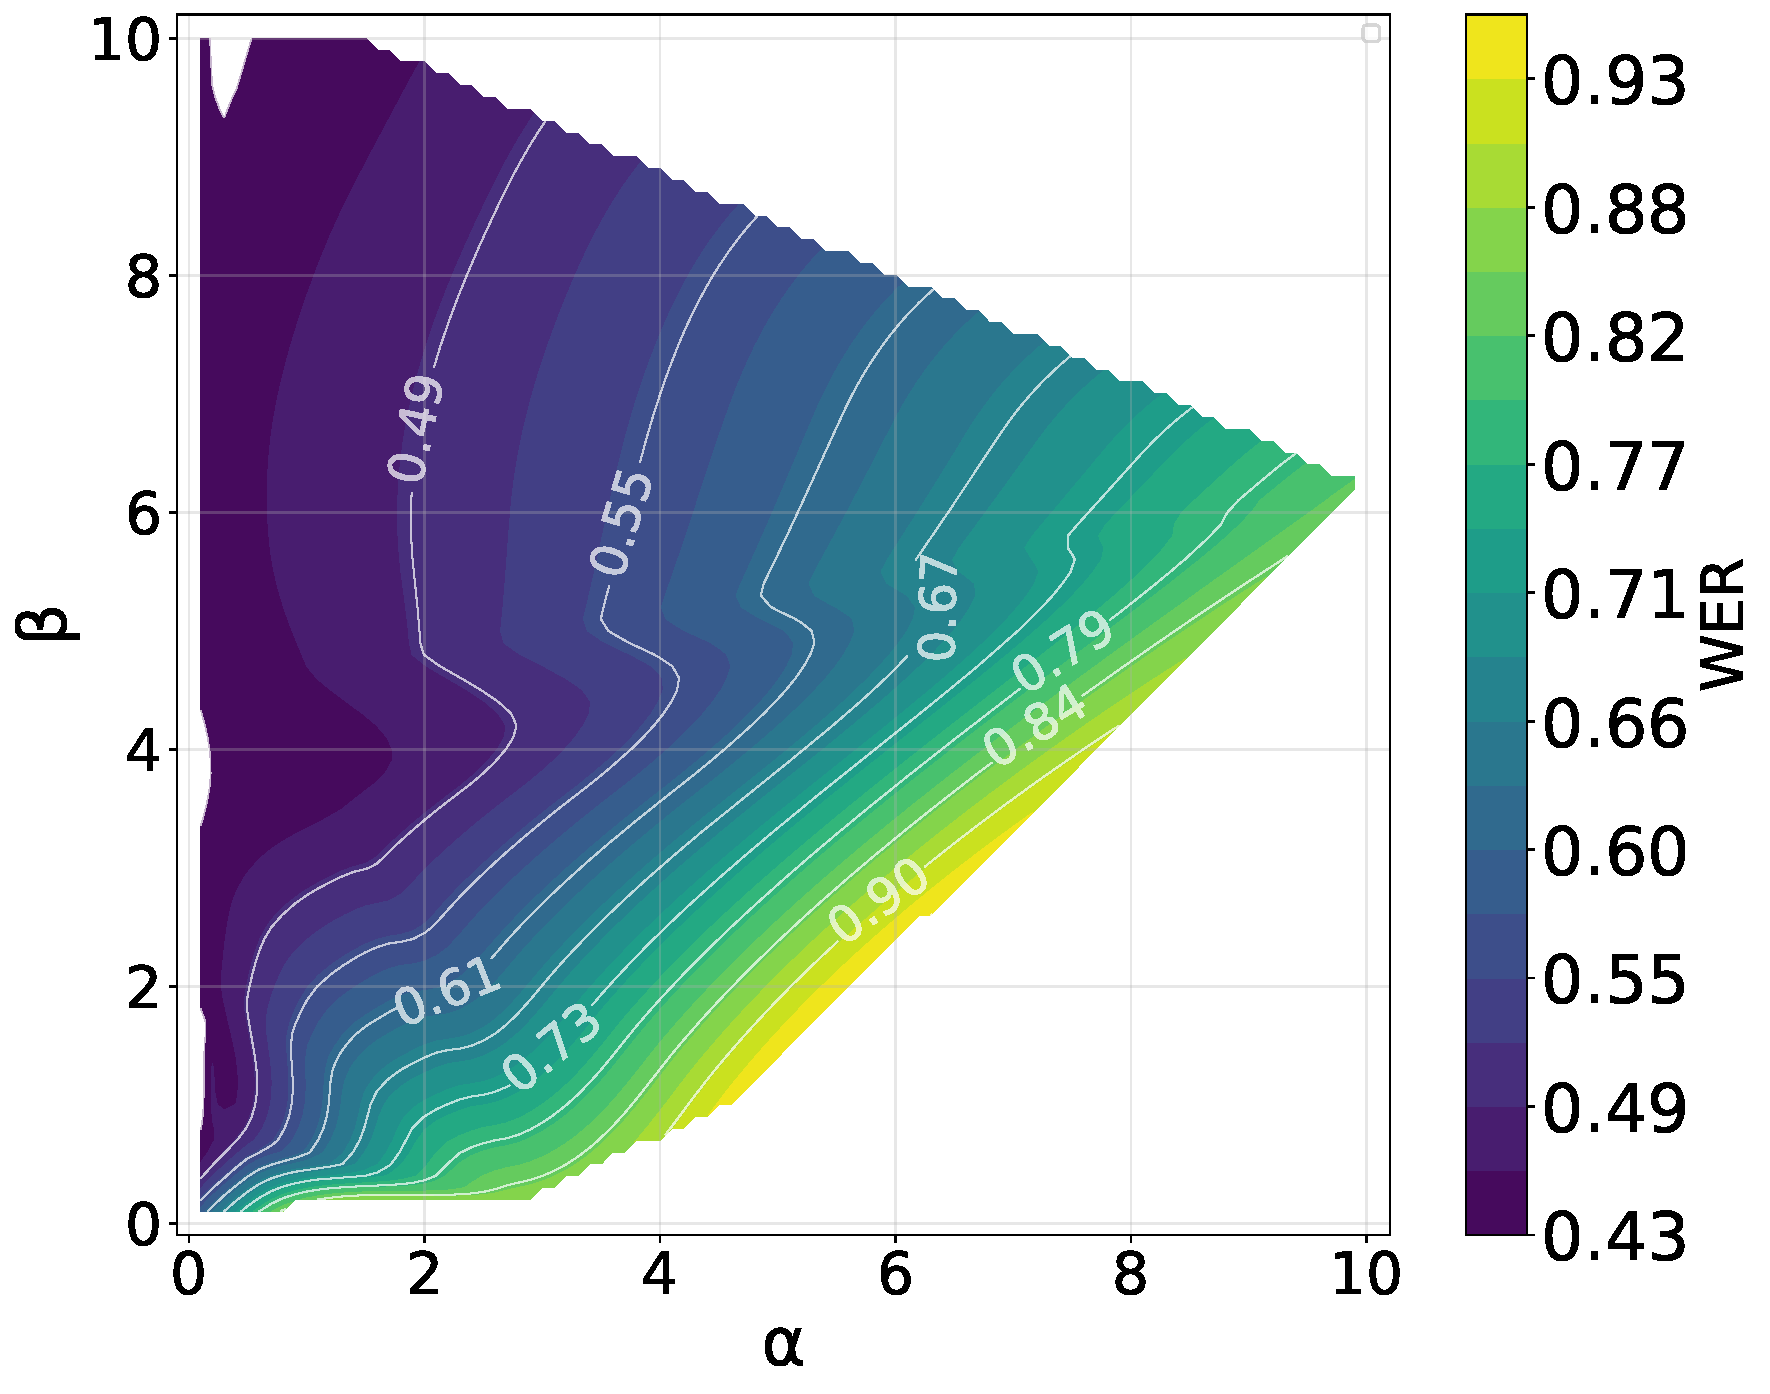
\includegraphics[width=0.9\linewidth]{papers/BaldWhisper/images/isoloss_wer_plot.pdf}
    \caption{Choice of \(\alpha\) and \(\beta\). Bayesian hyperparameter search indicates that the main constraint is to keep the lower-layer weight \(\alpha\) small.}
    \label{fig:convergence-bw}
\end{figure}

\paragraph{Why merge adjacent layers?}
Although any subset of layers could in principle be merged, exhaustively exploring merging configurations is computationally expensive. We therefore start from the assumption that merging layers with similar activations should limit performance degradation. We compute decoder-layer activations by forwarding the supervised validation corpus through Whisper-base, then compare every pair of layers. Figure~\ref{fig:similarities-bw} shows that adjacent layers tend to have similar activations, supporting the decision to merge consecutive pairs.

\begin{figure}[ht]
    \centering
    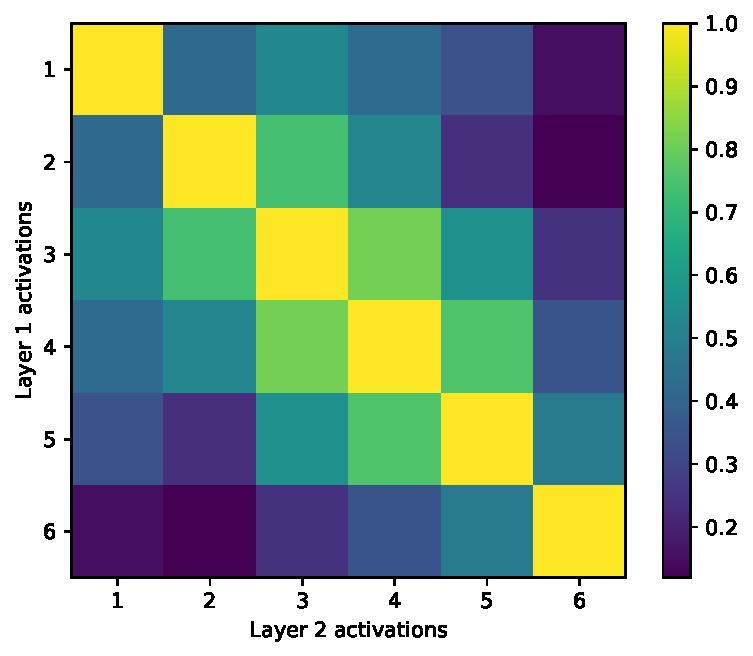
\includegraphics[width=0.9\linewidth]{papers/BaldWhisper/images/layer_similaritues.pdf}
    \caption{Activation similarities between all decoder-layer pairs. Consecutive layers tend to be more similar, suggesting that they can be merged.}
    \label{fig:similarities-bw}
\end{figure}

\paragraph{Comparison to brute-force search.}
One approach is to search which layer to remove by testing all combinations. Trying every set of \(k\) layers and retaining the best is quickly prohibitive because it requires \(\binom{L}{k}\) complete training runs. For Whisper-large with \(L=32\) and \(k=3\), this would require \(\binom{32}{3}=4960\) runs.
On the other side, with our approach, 10 to 20 small training runs are sufficient to determine the
weights of layer merging.

\paragraph{Confidence intervals.}
At a \(1.54\times\) speedup, layer merging obtains a WER of \(34.77\%\pm2.44\%\), statistically indistinguishable from the \(33.11\%\pm2.41\%\) baseline. Even at a \(2.15\times\) speedup, the WER of \(36.49\%\pm2.47\%\) represents a modest and predictable degradation.

\section{Extreme Head Shearing of LLMs}
So far, we have studied compression only on Whisper, but the same process can be applied to
autoregressive language models. Compressing the input/output embedding is particularly
justified for recent small language models, where it can account for up to 50\% of the total
parameters. We compressed Qwen2.5-0.5B and Gemma3-270M-it by reducing the number of parameters
in their tied input/output embeddings by $4\times$. For Gemma3-270M-it, this results
in a model with 140M parameters, roughly 50\% smaller than the original. We then applied
a short recovery fine-tuning stage on the smol-smoltalk corpus, using a language modeling
loss without knowledge distillation.

Figure~\ref{fig:baldqwen-training-loss} compares the training loss of the compressed and
non-compressed Qwen2.5-0.5B models. We can see that the compressed model converges well,
with both models reaching a loss of approximately 1.10.
Table~\ref{tab:gemma-head-shearing} compares the evaluation results of the compressed
Gemma3-270M-it model with those of the non-compressed model. Although compression degrades
performance, longer fine-tuning combined with knowledge distillation could help recover
some of the lost performance.

\begin{table}[!ht]
    \centering
    \begin{tabular}{lcc}
    \toprule
    \textbf{Benchmark} & \textbf{Gemma} & \textbf{Compressed Gemma} \\
    \midrule
    HellaSwag & 38.90 & 26.80 \\
    BoolQ & 55.72 & 41.99 \\
    PIQA & 66.81 & 51.80 \\
    ARC-Challenge & 27.73 & 24.23 \\
    WinoGrande & 52.17 & 47.99 \\
    \bottomrule
    \end{tabular}
    \caption{\textbf{Extreme head shearing of Gemma.} Scores are percentages
    (higher is better). We report normalized accuracy for HellaSwag, PIQA,
    and ARC-Challenge, and accuracy for BoolQ and WinoGrande.}
    \label{tab:gemma-head-shearing}
\end{table}

\begin{figure}[!ht]
    \centering
    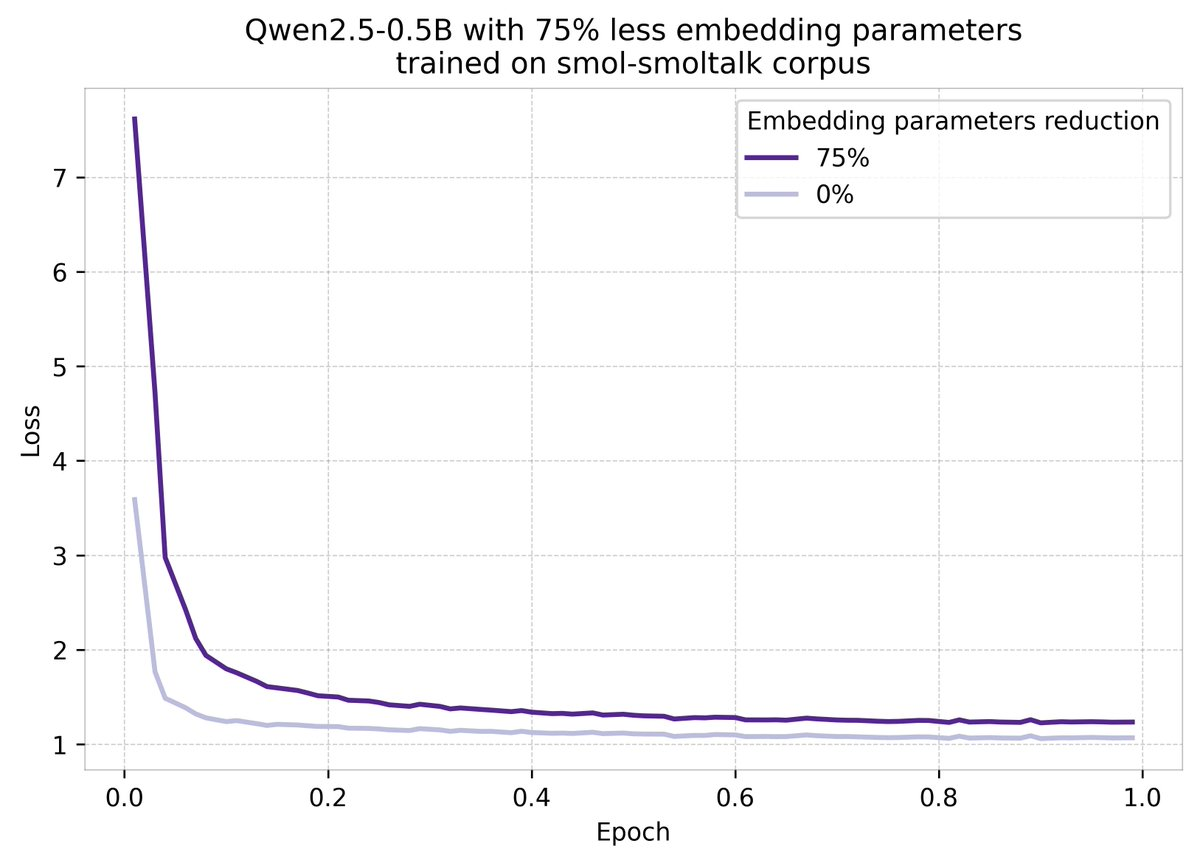
\includegraphics[width=\linewidth]{figures/baldqwen.jpg}
    \caption{Training loss of Qwen2.5-0.5B on the smol-smoltalk corpus,
    comparing a 75\% reduction in embedding parameters with the uncompressed
    baseline.}
    \label{fig:baldqwen-training-loss}
\end{figure}

\section{Conclusion}

We introduced BaldWhisper, a compression approach for Whisper in low-resource settings. Merging adjacent decoder layers rather than simply pruning them limits the performance loss, while low-rank feature distillation compresses the large shared embedding matrix without discarding vocabulary items needed for code-switching. Using only 32 hours of Bambara speech, the final model is \(2.15\times\) faster and 48\% smaller than Whisper-base while retaining more than 90\% of its performance.

Several directions could further improve this tradeoff. The merging weights \(\alpha\) and \(\beta\) could be specialized per layer, and more sophisticated merging functions~\citep{yadav2023tiesmergingresolvinginterferencemerging,yu2024languagemodelssupermario} could replace the weighted average. Because the method operates on standard Whisper Transformer blocks, it should transfer to other languages; validating that transfer remains future work.
